% Created by tikzDevice version 0.12 on 2019-09-25 12:21:47
% !TEX encoding = UTF-8 Unicode
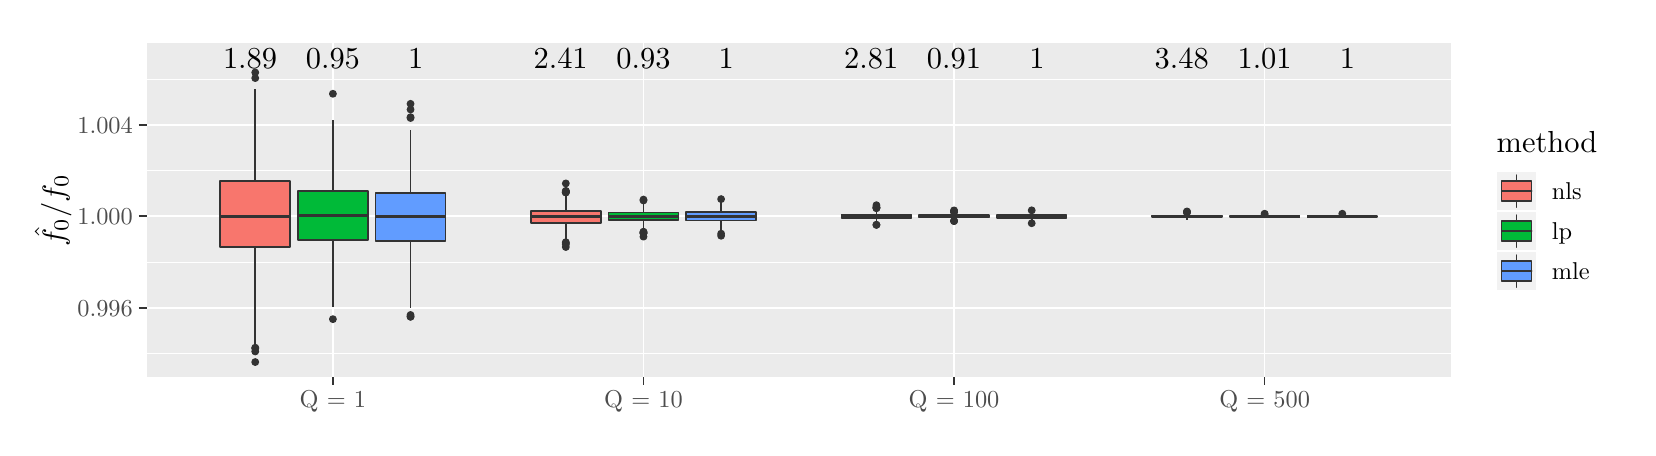
\begin{tikzpicture}[x=1pt,y=1pt]
\definecolor{fillColor}{RGB}{255,255,255}
\path[use as bounding box,fill=fillColor,fill opacity=0.00] (0,0) rectangle (578.16,144.54);
\begin{scope}
\path[clip] (  0.00,  0.00) rectangle (578.16,144.54);
\definecolor{drawColor}{RGB}{255,255,255}
\definecolor{fillColor}{RGB}{255,255,255}

\path[draw=drawColor,line width= 0.6pt,line join=round,line cap=round,fill=fillColor] (  0.00,  0.00) rectangle (578.16,144.54);
\end{scope}
\begin{scope}
\path[clip] ( 42.95, 18.22) rectangle (514.31,139.04);
\definecolor{fillColor}{gray}{0.92}

\path[fill=fillColor] ( 42.95, 18.22) rectangle (514.31,139.04);
\definecolor{drawColor}{RGB}{255,255,255}

\path[draw=drawColor,line width= 0.3pt,line join=round] ( 42.95, 26.80) --
	(514.31, 26.80);

\path[draw=drawColor,line width= 0.3pt,line join=round] ( 42.95, 59.87) --
	(514.31, 59.87);

\path[draw=drawColor,line width= 0.3pt,line join=round] ( 42.95, 92.93) --
	(514.31, 92.93);

\path[draw=drawColor,line width= 0.3pt,line join=round] ( 42.95,126.00) --
	(514.31,126.00);

\path[draw=drawColor,line width= 0.6pt,line join=round] ( 42.95, 43.34) --
	(514.31, 43.34);

\path[draw=drawColor,line width= 0.6pt,line join=round] ( 42.95, 76.40) --
	(514.31, 76.40);

\path[draw=drawColor,line width= 0.6pt,line join=round] ( 42.95,109.47) --
	(514.31,109.47);

\path[draw=drawColor,line width= 0.6pt,line join=round] (110.29, 18.22) --
	(110.29,139.04);

\path[draw=drawColor,line width= 0.6pt,line join=round] (222.52, 18.22) --
	(222.52,139.04);

\path[draw=drawColor,line width= 0.6pt,line join=round] (334.74, 18.22) --
	(334.74,139.04);

\path[draw=drawColor,line width= 0.6pt,line join=round] (446.97, 18.22) --
	(446.97,139.04);
\definecolor{drawColor}{gray}{0.20}
\definecolor{fillColor}{gray}{0.20}

\path[draw=drawColor,line width= 0.4pt,line join=round,line cap=round,fill=fillColor] ( 82.23, 27.54) circle (  1.21);

\path[draw=drawColor,line width= 0.4pt,line join=round,line cap=round,fill=fillColor] ( 82.23, 28.64) circle (  1.21);

\path[draw=drawColor,line width= 0.4pt,line join=round,line cap=round,fill=fillColor] ( 82.23,126.32) circle (  1.21);

\path[draw=drawColor,line width= 0.4pt,line join=round,line cap=round,fill=fillColor] ( 82.23, 28.90) circle (  1.21);

\path[draw=drawColor,line width= 0.4pt,line join=round,line cap=round,fill=fillColor] ( 82.23,128.35) circle (  1.21);

\path[draw=drawColor,line width= 0.4pt,line join=round,line cap=round,fill=fillColor] ( 82.23, 23.71) circle (  1.21);

\path[draw=drawColor,line width= 0.6pt,line join=round] ( 82.23, 89.19) -- ( 82.23,122.52);

\path[draw=drawColor,line width= 0.6pt,line join=round] ( 82.23, 65.24) -- ( 82.23, 29.84);
\definecolor{fillColor}{RGB}{248,118,109}

\path[draw=drawColor,line width= 0.6pt,line join=round,line cap=round,fill=fillColor] ( 69.61, 89.19) --
	( 69.61, 65.24) --
	( 94.86, 65.24) --
	( 94.86, 89.19) --
	( 69.61, 89.19) --
	cycle;

\path[draw=drawColor,line width= 1.1pt,line join=round] ( 69.61, 76.38) -- ( 94.86, 76.38);
\definecolor{fillColor}{gray}{0.20}

\path[draw=drawColor,line width= 0.4pt,line join=round,line cap=round,fill=fillColor] (110.29,120.65) circle (  1.21);

\path[draw=drawColor,line width= 0.4pt,line join=round,line cap=round,fill=fillColor] (110.29, 39.21) circle (  1.21);

\path[draw=drawColor,line width= 0.6pt,line join=round] (110.29, 85.51) -- (110.29,111.08);

\path[draw=drawColor,line width= 0.6pt,line join=round] (110.29, 67.77) -- (110.29, 43.56);
\definecolor{fillColor}{RGB}{0,186,56}

\path[draw=drawColor,line width= 0.6pt,line join=round,line cap=round,fill=fillColor] ( 97.66, 85.51) --
	( 97.66, 67.77) --
	(122.92, 67.77) --
	(122.92, 85.51) --
	( 97.66, 85.51) --
	cycle;

\path[draw=drawColor,line width= 1.1pt,line join=round] ( 97.66, 76.56) -- (122.92, 76.56);
\definecolor{fillColor}{gray}{0.20}

\path[draw=drawColor,line width= 0.4pt,line join=round,line cap=round,fill=fillColor] (138.35,117.02) circle (  1.21);

\path[draw=drawColor,line width= 0.4pt,line join=round,line cap=round,fill=fillColor] (138.35,112.20) circle (  1.21);

\path[draw=drawColor,line width= 0.4pt,line join=round,line cap=round,fill=fillColor] (138.35, 40.07) circle (  1.21);

\path[draw=drawColor,line width= 0.4pt,line join=round,line cap=round,fill=fillColor] (138.35,111.89) circle (  1.21);

\path[draw=drawColor,line width= 0.4pt,line join=round,line cap=round,fill=fillColor] (138.35, 40.73) circle (  1.21);

\path[draw=drawColor,line width= 0.4pt,line join=round,line cap=round,fill=fillColor] (138.35,114.97) circle (  1.21);

\path[draw=drawColor,line width= 0.4pt,line join=round,line cap=round,fill=fillColor] (138.35, 40.12) circle (  1.21);

\path[draw=drawColor,line width= 0.6pt,line join=round] (138.35, 84.87) -- (138.35,107.56);

\path[draw=drawColor,line width= 0.6pt,line join=round] (138.35, 67.48) -- (138.35, 43.35);
\definecolor{fillColor}{RGB}{97,156,255}

\path[draw=drawColor,line width= 0.6pt,line join=round,line cap=round,fill=fillColor] (125.72, 84.87) --
	(125.72, 67.48) --
	(150.97, 67.48) --
	(150.97, 84.87) --
	(125.72, 84.87) --
	cycle;

\path[draw=drawColor,line width= 1.1pt,line join=round] (125.72, 76.40) -- (150.97, 76.40);
\definecolor{fillColor}{gray}{0.20}

\path[draw=drawColor,line width= 0.4pt,line join=round,line cap=round,fill=fillColor] (194.46, 66.67) circle (  1.21);

\path[draw=drawColor,line width= 0.4pt,line join=round,line cap=round,fill=fillColor] (194.46, 65.28) circle (  1.21);

\path[draw=drawColor,line width= 0.4pt,line join=round,line cap=round,fill=fillColor] (194.46, 88.26) circle (  1.21);

\path[draw=drawColor,line width= 0.4pt,line join=round,line cap=round,fill=fillColor] (194.46, 85.48) circle (  1.21);

\path[draw=drawColor,line width= 0.4pt,line join=round,line cap=round,fill=fillColor] (194.46, 85.19) circle (  1.21);

\path[draw=drawColor,line width= 0.4pt,line join=round,line cap=round,fill=fillColor] (194.46, 84.99) circle (  1.21);

\path[draw=drawColor,line width= 0.4pt,line join=round,line cap=round,fill=fillColor] (194.46, 67.01) circle (  1.21);

\path[draw=drawColor,line width= 0.4pt,line join=round,line cap=round,fill=fillColor] (194.46, 66.25) circle (  1.21);

\path[draw=drawColor,line width= 0.4pt,line join=round,line cap=round,fill=fillColor] (194.46, 85.55) circle (  1.21);

\path[draw=drawColor,line width= 0.4pt,line join=round,line cap=round,fill=fillColor] (194.46, 85.02) circle (  1.21);

\path[draw=drawColor,line width= 0.4pt,line join=round,line cap=round,fill=fillColor] (194.46, 85.13) circle (  1.21);

\path[draw=drawColor,line width= 0.6pt,line join=round] (194.46, 78.33) -- (194.46, 84.81);

\path[draw=drawColor,line width= 0.6pt,line join=round] (194.46, 73.98) -- (194.46, 67.65);
\definecolor{fillColor}{RGB}{248,118,109}

\path[draw=drawColor,line width= 0.6pt,line join=round,line cap=round,fill=fillColor] (181.83, 78.33) --
	(181.83, 73.98) --
	(207.09, 73.98) --
	(207.09, 78.33) --
	(181.83, 78.33) --
	cycle;

\path[draw=drawColor,line width= 1.1pt,line join=round] (181.83, 76.18) -- (207.09, 76.18);
\definecolor{fillColor}{gray}{0.20}

\path[draw=drawColor,line width= 0.4pt,line join=round,line cap=round,fill=fillColor] (222.52, 69.03) circle (  1.21);

\path[draw=drawColor,line width= 0.4pt,line join=round,line cap=round,fill=fillColor] (222.52, 70.71) circle (  1.21);

\path[draw=drawColor,line width= 0.4pt,line join=round,line cap=round,fill=fillColor] (222.52, 70.30) circle (  1.21);

\path[draw=drawColor,line width= 0.4pt,line join=round,line cap=round,fill=fillColor] (222.52, 82.42) circle (  1.21);

\path[draw=drawColor,line width= 0.4pt,line join=round,line cap=round,fill=fillColor] (222.52, 70.18) circle (  1.21);

\path[draw=drawColor,line width= 0.4pt,line join=round,line cap=round,fill=fillColor] (222.52, 82.09) circle (  1.21);

\path[draw=drawColor,line width= 0.4pt,line join=round,line cap=round,fill=fillColor] (222.52, 70.79) circle (  1.21);

\path[draw=drawColor,line width= 0.4pt,line join=round,line cap=round,fill=fillColor] (222.52, 70.38) circle (  1.21);

\path[draw=drawColor,line width= 0.6pt,line join=round] (222.52, 77.79) -- (222.52, 81.84);

\path[draw=drawColor,line width= 0.6pt,line join=round] (222.52, 75.05) -- (222.52, 71.02);
\definecolor{fillColor}{RGB}{0,186,56}

\path[draw=drawColor,line width= 0.6pt,line join=round,line cap=round,fill=fillColor] (209.89, 77.79) --
	(209.89, 75.05) --
	(235.14, 75.05) --
	(235.14, 77.79) --
	(209.89, 77.79) --
	cycle;

\path[draw=drawColor,line width= 1.1pt,line join=round] (209.89, 76.40) -- (235.14, 76.40);
\definecolor{fillColor}{gray}{0.20}

\path[draw=drawColor,line width= 0.4pt,line join=round,line cap=round,fill=fillColor] (250.57, 69.35) circle (  1.21);

\path[draw=drawColor,line width= 0.4pt,line join=round,line cap=round,fill=fillColor] (250.57, 82.59) circle (  1.21);

\path[draw=drawColor,line width= 0.4pt,line join=round,line cap=round,fill=fillColor] (250.57, 70.09) circle (  1.21);

\path[draw=drawColor,line width= 0.6pt,line join=round] (250.57, 77.93) -- (250.57, 82.02);

\path[draw=drawColor,line width= 0.6pt,line join=round] (250.57, 74.85) -- (250.57, 70.59);
\definecolor{fillColor}{RGB}{97,156,255}

\path[draw=drawColor,line width= 0.6pt,line join=round,line cap=round,fill=fillColor] (237.95, 77.93) --
	(237.95, 74.85) --
	(263.20, 74.85) --
	(263.20, 77.93) --
	(237.95, 77.93) --
	cycle;

\path[draw=drawColor,line width= 1.1pt,line join=round] (237.95, 76.40) -- (263.20, 76.40);
\definecolor{fillColor}{gray}{0.20}

\path[draw=drawColor,line width= 0.4pt,line join=round,line cap=round,fill=fillColor] (306.69, 79.60) circle (  1.21);

\path[draw=drawColor,line width= 0.4pt,line join=round,line cap=round,fill=fillColor] (306.69, 73.32) circle (  1.21);

\path[draw=drawColor,line width= 0.4pt,line join=round,line cap=round,fill=fillColor] (306.69, 80.39) circle (  1.21);

\path[draw=drawColor,line width= 0.4pt,line join=round,line cap=round,fill=fillColor] (306.69, 79.38) circle (  1.21);

\path[draw=drawColor,line width= 0.4pt,line join=round,line cap=round,fill=fillColor] (306.69, 73.27) circle (  1.21);

\path[draw=drawColor,line width= 0.4pt,line join=round,line cap=round,fill=fillColor] (306.69, 79.30) circle (  1.21);

\path[draw=drawColor,line width= 0.4pt,line join=round,line cap=round,fill=fillColor] (306.69, 79.64) circle (  1.21);

\path[draw=drawColor,line width= 0.6pt,line join=round] (306.69, 77.05) -- (306.69, 79.09);

\path[draw=drawColor,line width= 0.6pt,line join=round] (306.69, 75.65) -- (306.69, 73.82);
\definecolor{fillColor}{RGB}{248,118,109}

\path[draw=drawColor,line width= 0.6pt,line join=round,line cap=round,fill=fillColor] (294.06, 77.05) --
	(294.06, 75.65) --
	(319.31, 75.65) --
	(319.31, 77.05) --
	(294.06, 77.05) --
	cycle;

\path[draw=drawColor,line width= 1.1pt,line join=round] (294.06, 76.35) -- (319.31, 76.35);
\definecolor{fillColor}{gray}{0.20}

\path[draw=drawColor,line width= 0.4pt,line join=round,line cap=round,fill=fillColor] (334.74, 78.52) circle (  1.21);

\path[draw=drawColor,line width= 0.4pt,line join=round,line cap=round,fill=fillColor] (334.74, 78.15) circle (  1.21);

\path[draw=drawColor,line width= 0.4pt,line join=round,line cap=round,fill=fillColor] (334.74, 78.11) circle (  1.21);

\path[draw=drawColor,line width= 0.4pt,line join=round,line cap=round,fill=fillColor] (334.74, 78.00) circle (  1.21);

\path[draw=drawColor,line width= 0.4pt,line join=round,line cap=round,fill=fillColor] (334.74, 74.67) circle (  1.21);

\path[draw=drawColor,line width= 0.4pt,line join=round,line cap=round,fill=fillColor] (334.74, 74.71) circle (  1.21);

\path[draw=drawColor,line width= 0.4pt,line join=round,line cap=round,fill=fillColor] (334.74, 74.68) circle (  1.21);

\path[draw=drawColor,line width= 0.4pt,line join=round,line cap=round,fill=fillColor] (334.74, 78.06) circle (  1.21);

\path[draw=drawColor,line width= 0.6pt,line join=round] (334.74, 76.77) -- (334.74, 77.98);

\path[draw=drawColor,line width= 0.6pt,line join=round] (334.74, 75.96) -- (334.74, 74.85);
\definecolor{fillColor}{RGB}{0,186,56}

\path[draw=drawColor,line width= 0.6pt,line join=round,line cap=round,fill=fillColor] (322.12, 76.77) --
	(322.12, 75.96) --
	(347.37, 75.96) --
	(347.37, 76.77) --
	(322.12, 76.77) --
	cycle;

\path[draw=drawColor,line width= 1.1pt,line join=round] (322.12, 76.35) -- (347.37, 76.35);
\definecolor{fillColor}{gray}{0.20}

\path[draw=drawColor,line width= 0.4pt,line join=round,line cap=round,fill=fillColor] (362.80, 73.88) circle (  1.21);

\path[draw=drawColor,line width= 0.4pt,line join=round,line cap=round,fill=fillColor] (362.80, 78.53) circle (  1.21);

\path[draw=drawColor,line width= 0.6pt,line join=round] (362.80, 76.82) -- (362.80, 78.11);

\path[draw=drawColor,line width= 0.6pt,line join=round] (362.80, 75.88) -- (362.80, 74.68);
\definecolor{fillColor}{RGB}{97,156,255}

\path[draw=drawColor,line width= 0.6pt,line join=round,line cap=round,fill=fillColor] (350.18, 76.82) --
	(350.18, 75.88) --
	(375.43, 75.88) --
	(375.43, 76.82) --
	(350.18, 76.82) --
	cycle;

\path[draw=drawColor,line width= 1.1pt,line join=round] (350.18, 76.40) -- (375.43, 76.40);
\definecolor{fillColor}{gray}{0.20}

\path[draw=drawColor,line width= 0.4pt,line join=round,line cap=round,fill=fillColor] (418.91, 78.13) circle (  1.21);

\path[draw=drawColor,line width= 0.4pt,line join=round,line cap=round,fill=fillColor] (418.91, 77.83) circle (  1.21);

\path[draw=drawColor,line width= 0.4pt,line join=round,line cap=round,fill=fillColor] (418.91, 77.73) circle (  1.21);

\path[draw=drawColor,line width= 0.4pt,line join=round,line cap=round,fill=fillColor] (418.91, 77.96) circle (  1.21);

\path[draw=drawColor,line width= 0.6pt,line join=round] (418.91, 76.71) -- (418.91, 77.62);

\path[draw=drawColor,line width= 0.6pt,line join=round] (418.91, 76.07) -- (418.91, 75.16);
\definecolor{fillColor}{RGB}{248,118,109}

\path[draw=drawColor,line width= 0.6pt,line join=round,line cap=round,fill=fillColor] (406.29, 76.71) --
	(406.29, 76.07) --
	(431.54, 76.07) --
	(431.54, 76.71) --
	(406.29, 76.71) --
	cycle;

\path[draw=drawColor,line width= 1.1pt,line join=round] (406.29, 76.41) -- (431.54, 76.41);
\definecolor{fillColor}{gray}{0.20}

\path[draw=drawColor,line width= 0.4pt,line join=round,line cap=round,fill=fillColor] (446.97, 77.30) circle (  1.21);

\path[draw=drawColor,line width= 0.4pt,line join=round,line cap=round,fill=fillColor] (446.97, 77.15) circle (  1.21);

\path[draw=drawColor,line width= 0.6pt,line join=round] (446.97, 76.58) -- (446.97, 77.09);

\path[draw=drawColor,line width= 0.6pt,line join=round] (446.97, 76.21) -- (446.97, 75.70);
\definecolor{fillColor}{RGB}{0,186,56}

\path[draw=drawColor,line width= 0.6pt,line join=round,line cap=round,fill=fillColor] (434.35, 76.58) --
	(434.35, 76.21) --
	(459.60, 76.21) --
	(459.60, 76.58) --
	(434.35, 76.58) --
	cycle;

\path[draw=drawColor,line width= 1.1pt,line join=round] (434.35, 76.39) -- (459.60, 76.39);
\definecolor{fillColor}{gray}{0.20}

\path[draw=drawColor,line width= 0.4pt,line join=round,line cap=round,fill=fillColor] (475.03, 77.31) circle (  1.21);

\path[draw=drawColor,line width= 0.6pt,line join=round] (475.03, 76.58) -- (475.03, 77.11);

\path[draw=drawColor,line width= 0.6pt,line join=round] (475.03, 76.20) -- (475.03, 75.72);
\definecolor{fillColor}{RGB}{97,156,255}

\path[draw=drawColor,line width= 0.6pt,line join=round,line cap=round,fill=fillColor] (462.40, 76.58) --
	(462.40, 76.20) --
	(487.65, 76.20) --
	(487.65, 76.58) --
	(462.40, 76.58) --
	cycle;

\path[draw=drawColor,line width= 1.1pt,line join=round] (462.40, 76.40) -- (487.65, 76.40);
\definecolor{drawColor}{RGB}{0,0,0}

\node[text=drawColor,anchor=base,inner sep=0pt, outer sep=0pt, scale=  1.10] at (140.22,129.75) {1};

\node[text=drawColor,anchor=base,inner sep=0pt, outer sep=0pt, scale=  1.10] at (110.29,129.75) {0.95};

\node[text=drawColor,anchor=base,inner sep=0pt, outer sep=0pt, scale=  1.10] at ( 80.36,129.75) {1.89};

\node[text=drawColor,anchor=base,inner sep=0pt, outer sep=0pt, scale=  1.10] at (252.44,129.75) {1};

\node[text=drawColor,anchor=base,inner sep=0pt, outer sep=0pt, scale=  1.10] at (222.52,129.75) {0.93};

\node[text=drawColor,anchor=base,inner sep=0pt, outer sep=0pt, scale=  1.10] at (192.59,129.75) {2.41};

\node[text=drawColor,anchor=base,inner sep=0pt, outer sep=0pt, scale=  1.10] at (364.67,129.75) {1};

\node[text=drawColor,anchor=base,inner sep=0pt, outer sep=0pt, scale=  1.10] at (334.74,129.75) {0.91};

\node[text=drawColor,anchor=base,inner sep=0pt, outer sep=0pt, scale=  1.10] at (304.82,129.75) {2.81};

\node[text=drawColor,anchor=base,inner sep=0pt, outer sep=0pt, scale=  1.10] at (476.90,129.75) {1};

\node[text=drawColor,anchor=base,inner sep=0pt, outer sep=0pt, scale=  1.10] at (446.97,129.75) {1.01};

\node[text=drawColor,anchor=base,inner sep=0pt, outer sep=0pt, scale=  1.10] at (417.04,129.75) {3.48};
\end{scope}
\begin{scope}
\path[clip] (  0.00,  0.00) rectangle (578.16,144.54);
\definecolor{drawColor}{gray}{0.30}

\node[text=drawColor,anchor=base east,inner sep=0pt, outer sep=0pt, scale=  0.88] at ( 38.00, 40.30) {0.996};

\node[text=drawColor,anchor=base east,inner sep=0pt, outer sep=0pt, scale=  0.88] at ( 38.00, 73.37) {1.000};

\node[text=drawColor,anchor=base east,inner sep=0pt, outer sep=0pt, scale=  0.88] at ( 38.00,106.44) {1.004};
\end{scope}
\begin{scope}
\path[clip] (  0.00,  0.00) rectangle (578.16,144.54);
\definecolor{drawColor}{gray}{0.20}

\path[draw=drawColor,line width= 0.6pt,line join=round] ( 40.20, 43.34) --
	( 42.95, 43.34);

\path[draw=drawColor,line width= 0.6pt,line join=round] ( 40.20, 76.40) --
	( 42.95, 76.40);

\path[draw=drawColor,line width= 0.6pt,line join=round] ( 40.20,109.47) --
	( 42.95,109.47);
\end{scope}
\begin{scope}
\path[clip] (  0.00,  0.00) rectangle (578.16,144.54);
\definecolor{drawColor}{gray}{0.20}

\path[draw=drawColor,line width= 0.6pt,line join=round] (110.29, 15.47) --
	(110.29, 18.22);

\path[draw=drawColor,line width= 0.6pt,line join=round] (222.52, 15.47) --
	(222.52, 18.22);

\path[draw=drawColor,line width= 0.6pt,line join=round] (334.74, 15.47) --
	(334.74, 18.22);

\path[draw=drawColor,line width= 0.6pt,line join=round] (446.97, 15.47) --
	(446.97, 18.22);
\end{scope}
\begin{scope}
\path[clip] (  0.00,  0.00) rectangle (578.16,144.54);
\definecolor{drawColor}{gray}{0.30}

\node[text=drawColor,anchor=base,inner sep=0pt, outer sep=0pt, scale=  0.88] at (110.29,  7.21) {Q = 1};

\node[text=drawColor,anchor=base,inner sep=0pt, outer sep=0pt, scale=  0.88] at (222.52,  7.21) {Q = 10};

\node[text=drawColor,anchor=base,inner sep=0pt, outer sep=0pt, scale=  0.88] at (334.74,  7.21) {Q = 100};

\node[text=drawColor,anchor=base,inner sep=0pt, outer sep=0pt, scale=  0.88] at (446.97,  7.21) {Q = 500};
\end{scope}
\begin{scope}
\path[clip] (  0.00,  0.00) rectangle (578.16,144.54);
\definecolor{drawColor}{RGB}{0,0,0}

\node[text=drawColor,rotate= 90.00,anchor=base,inner sep=0pt, outer sep=0pt, scale=  1.10] at ( 13.08, 78.63) {$\hat{f_0}/f_0$};
\end{scope}
\begin{scope}
\path[clip] (  0.00,  0.00) rectangle (578.16,144.54);
\definecolor{fillColor}{RGB}{255,255,255}

\path[fill=fillColor] (525.31, 43.84) rectangle (572.66,113.42);
\end{scope}
\begin{scope}
\path[clip] (  0.00,  0.00) rectangle (578.16,144.54);
\definecolor{drawColor}{RGB}{0,0,0}

\node[text=drawColor,anchor=base west,inner sep=0pt, outer sep=0pt, scale=  1.10] at (530.81, 99.27) {method};
\end{scope}
\begin{scope}
\path[clip] (  0.00,  0.00) rectangle (578.16,144.54);
\definecolor{drawColor}{RGB}{255,255,255}
\definecolor{fillColor}{gray}{0.95}

\path[draw=drawColor,line width= 0.6pt,line join=round,line cap=round,fill=fillColor] (530.81, 78.25) rectangle (545.26, 92.70);
\end{scope}
\begin{scope}
\path[clip] (  0.00,  0.00) rectangle (578.16,144.54);
\definecolor{drawColor}{gray}{0.20}

\path[draw=drawColor,line width= 0.6pt,line join=round,line cap=round] (538.03, 79.70) --
	(538.03, 81.86);

\path[draw=drawColor,line width= 0.6pt,line join=round,line cap=round] (538.03, 89.09) --
	(538.03, 91.26);
\definecolor{fillColor}{RGB}{248,118,109}

\path[draw=drawColor,line width= 0.6pt,line join=round,line cap=round,fill=fillColor] (532.61, 81.86) rectangle (543.45, 89.09);

\path[draw=drawColor,line width= 0.6pt,line join=round,line cap=round] (532.61, 85.48) --
	(543.45, 85.48);
\end{scope}
\begin{scope}
\path[clip] (  0.00,  0.00) rectangle (578.16,144.54);
\definecolor{drawColor}{RGB}{255,255,255}
\definecolor{fillColor}{gray}{0.95}

\path[draw=drawColor,line width= 0.6pt,line join=round,line cap=round,fill=fillColor] (530.81, 63.80) rectangle (545.26, 78.25);
\end{scope}
\begin{scope}
\path[clip] (  0.00,  0.00) rectangle (578.16,144.54);
\definecolor{drawColor}{gray}{0.20}

\path[draw=drawColor,line width= 0.6pt,line join=round,line cap=round] (538.03, 65.24) --
	(538.03, 67.41);

\path[draw=drawColor,line width= 0.6pt,line join=round,line cap=round] (538.03, 74.64) --
	(538.03, 76.81);
\definecolor{fillColor}{RGB}{0,186,56}

\path[draw=drawColor,line width= 0.6pt,line join=round,line cap=round,fill=fillColor] (532.61, 67.41) rectangle (543.45, 74.64);

\path[draw=drawColor,line width= 0.6pt,line join=round,line cap=round] (532.61, 71.02) --
	(543.45, 71.02);
\end{scope}
\begin{scope}
\path[clip] (  0.00,  0.00) rectangle (578.16,144.54);
\definecolor{drawColor}{RGB}{255,255,255}
\definecolor{fillColor}{gray}{0.95}

\path[draw=drawColor,line width= 0.6pt,line join=round,line cap=round,fill=fillColor] (530.81, 49.34) rectangle (545.26, 63.80);
\end{scope}
\begin{scope}
\path[clip] (  0.00,  0.00) rectangle (578.16,144.54);
\definecolor{drawColor}{gray}{0.20}

\path[draw=drawColor,line width= 0.6pt,line join=round,line cap=round] (538.03, 50.79) --
	(538.03, 52.96);

\path[draw=drawColor,line width= 0.6pt,line join=round,line cap=round] (538.03, 60.18) --
	(538.03, 62.35);
\definecolor{fillColor}{RGB}{97,156,255}

\path[draw=drawColor,line width= 0.6pt,line join=round,line cap=round,fill=fillColor] (532.61, 52.96) rectangle (543.45, 60.18);

\path[draw=drawColor,line width= 0.6pt,line join=round,line cap=round] (532.61, 56.57) --
	(543.45, 56.57);
\end{scope}
\begin{scope}
\path[clip] (  0.00,  0.00) rectangle (578.16,144.54);
\definecolor{drawColor}{RGB}{0,0,0}

\node[text=drawColor,anchor=base west,inner sep=0pt, outer sep=0pt, scale=  0.88] at (550.76, 82.45) {nls};
\end{scope}
\begin{scope}
\path[clip] (  0.00,  0.00) rectangle (578.16,144.54);
\definecolor{drawColor}{RGB}{0,0,0}

\node[text=drawColor,anchor=base west,inner sep=0pt, outer sep=0pt, scale=  0.88] at (550.76, 67.99) {lp};
\end{scope}
\begin{scope}
\path[clip] (  0.00,  0.00) rectangle (578.16,144.54);
\definecolor{drawColor}{RGB}{0,0,0}

\node[text=drawColor,anchor=base west,inner sep=0pt, outer sep=0pt, scale=  0.88] at (550.76, 53.54) {mle};
\end{scope}
\end{tikzpicture}
